\documentclass[tikz,class=minimal,border=0pt,12pt]{standalone}

\makeatletter
\tikzset{pics/named scope code/.style={code={\tikz@fig@mustbenamed%
      \begin{scope}[local bounding box/.expanded=\tikz@fig@name]#1\end{scope}%
    }}}

\usepackage{ifthen}
\usepackage{marvosym}
\usepackage{etoolbox}
\usepackage{multido}
\usepackage{fontspec}
\setmainfont{Arial}

\newcommand*{\rom}[1]{\expandafter\@slowromancap\romannumeral #1@}

\definecolor{treatment}{rgb}{0.37,0.23,0.53}
\definecolor{placebo}{rgb}{0.90,0.38,0.003}

\tikzset{
  smallBox/.style = {draw, gray, inner xsep=-0.25em, inner ysep=-0.25em},
  textNode/.style = {align=left, anchor=west}
}

\usetikzlibrary{calc, datavisualization,
  datavisualization.formats.functions,  
  fit, math, positioning, shapes}

\begin{document}
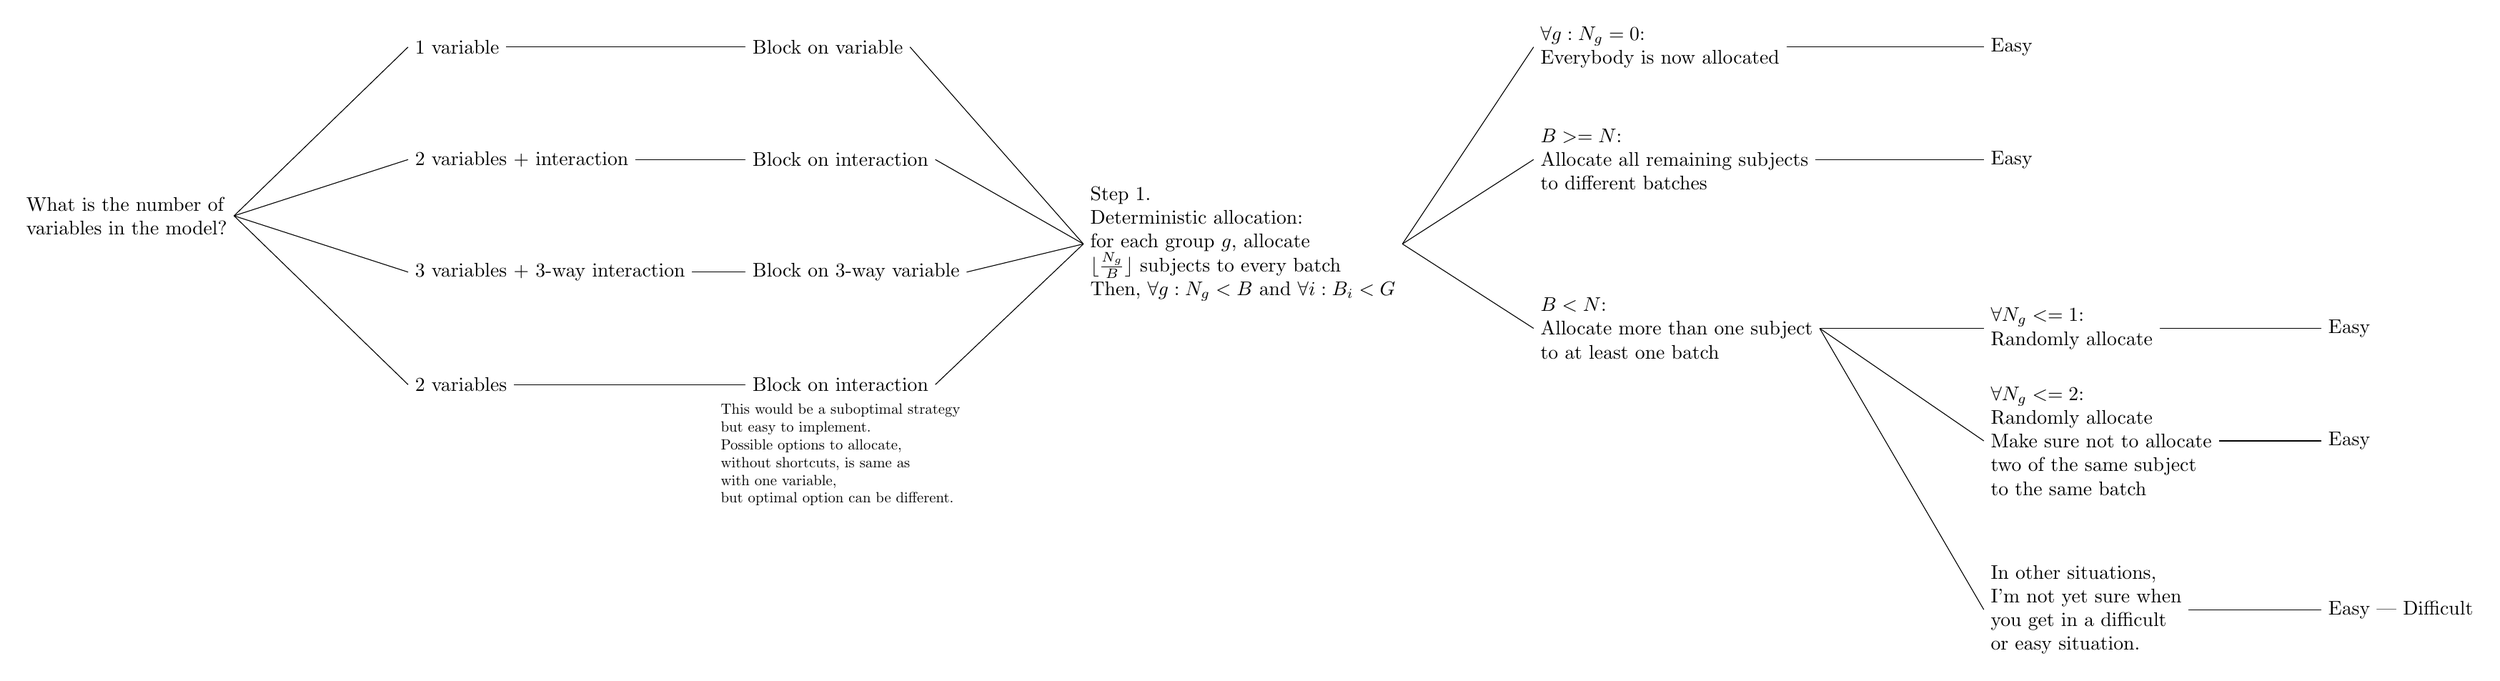
\begin{tikzpicture}
  \node[textNode] (nVar) at (0,0) {What is the number of\\ variables in the model?};

  \node[textNode] (oneVar) at ($(nVar) + (5, 3)$) {1 variable};
  \draw (nVar.east) -- (oneVar.west);
  
  \node[textNode] (twoVarInt) at ($(nVar) + (5, 1)$) {2 variables + interaction};
  \draw (nVar.east) -- (twoVarInt.west);
  
  \node[textNode] (threeVarThreeInt) at ($(nVar) + (5, -1)$) {3 variables + 3-way interaction};
  \draw (nVar.east) -- (threeVarThreeInt.west);
  
  \node[textNode] (twoVar) at ($(nVar) + (5, -3)$) {2 variables};
  \draw (nVar.east) -- (twoVar.west);

  \edef\blockOnD{6};
  \node[textNode] (oneVarBlockOn)  at ($(oneVar.west) + (\blockOnD, 0)$) {Block on variable};
  \node[textNode] (twoVarIntBlockOn)  at ($(twoVarInt.west) + (\blockOnD, 0)$) {Block on interaction};
  \node[textNode] (threeVarThreeIntBlockOn)  at ($(threeVarThreeInt.west) + (\blockOnD, 0)$) {Block on 3-way variable};
  \node[textNode] (twoVarBlockOn)  at ($(twoVar.west) + (\blockOnD, 0)$) {Block on interaction};
  \node[textNode, scale=.75, below= 0 of twoVarBlockOn] {This would be a suboptimal strategy\\but easy to implement.\\Possible options to allocate,\\ without shortcuts, is same as\\with one variable,\\but optimal option can be different.};
  \draw (oneVar.east) -- (oneVarBlockOn.west);
  \draw (twoVarInt.east) -- (twoVarIntBlockOn.west);
  \draw (threeVarThreeInt.east) -- (threeVarThreeIntBlockOn.west);
  \draw (twoVar.east) -- (twoVarBlockOn.west);

  \node[textNode] (stepOne)  at ($(twoVarIntBlockOn.west) + (\blockOnD, -1.5)$) {
    Step 1.\\ Deterministic allocation:\\ for each group $g$, allocate\\ $\lfloor\frac{N_g}{B}\rfloor$ subjects to every batch\\
    Then, $\forall g: N_g < B$ and $\forall i: B_i < G$
  };

  \draw [-] (oneVarBlockOn.east) -- (stepOne.west);
  \draw [-] (twoVarIntBlockOn.east) -- (stepOne.west);
  \draw [-] (threeVarThreeIntBlockOn.east) -- (stepOne.west);
  \draw [-] (twoVarBlockOn.east) -- (stepOne.west);

  
  \node[textNode] (done) at ($(stepOne.west) + (\blockOnD + 2, 3.5)$) {$\forall g: N_g = 0$: \\Everybody is now allocated};
  \draw (stepOne.east) -- (done.west);

  \node[textNode] (alloOne) at ($(stepOne.west) + (\blockOnD + 2, 1.5)$) {$B >= N$: \\Allocate all remaining subjects\\ to different batches};
  \draw (stepOne.east) -- (alloOne.west);

  \node[textNode] (doneEasy) at ($(done.west) + (\blockOnD + 2, 0)$) {Easy};
  \draw (done.east) -- (doneEasy.west);

  \node[textNode] (alloOneEasy) at ($(alloOne.west) + (\blockOnD + 2, 0)$) {Easy};
  \draw (alloOne.east) -- (alloOneEasy.west);

  \node[textNode] (alloMult) at ($(stepOne.west) + (\blockOnD + 2, -1.5)$) {$B < N$: \\Allocate more than one subject\\to at least one batch};
  \draw (stepOne.east) -- (alloMult.west);

  \node[textNode] (alloOnePerGroup) at ($(alloMult.west) + (\blockOnD + 2, 0)$) {$\forall N_g <= 1$: \\Randomly allocate};
  \draw (alloMult.east) -- (alloOnePerGroup.west);

  \node[textNode] (alloMaxTwoPerGroup) at ($(alloMult.west) + (\blockOnD + 2, -2)$) {$\forall N_g <= 2$: \\Randomly allocate\\Make sure not to allocate\\ two of the same subject\\ to the same batch};
  \draw (alloMult.east) -- (alloMaxTwoPerGroup.west);

  \node[textNode] (alloMany) at ($(alloMult.west) + (\blockOnD + 2, -5)$) {In other situations,\\I'm not yet sure when\\you get in a difficult\\or easy situation.};
  \draw (alloMult.east) -- (alloMany.west);

  \node[textNode] (alloOnePerGroupEasy) at ($(alloOnePerGroup.west) + (\blockOnD, 0)$) {Easy};
  \draw (alloOnePerGroup.east) -- (alloOnePerGroupEasy.west);

  \node[textNode] (alloMaxTwoPerGroupEasy) at ($(alloMaxTwoPerGroup.west) + (\blockOnD, 0)$) {Easy};
  \draw (alloMaxTwoPerGroup.east) -- (alloMaxTwoPerGroupEasy.west);

  \node[textNode] (alloManyEasy) at ($(alloMany.west) + (\blockOnD, 0)$) {Easy --- Difficult};
  \draw (alloMany.east) -- (alloManyEasy.west);
  
  
  
\end{tikzpicture}
\end{document}
